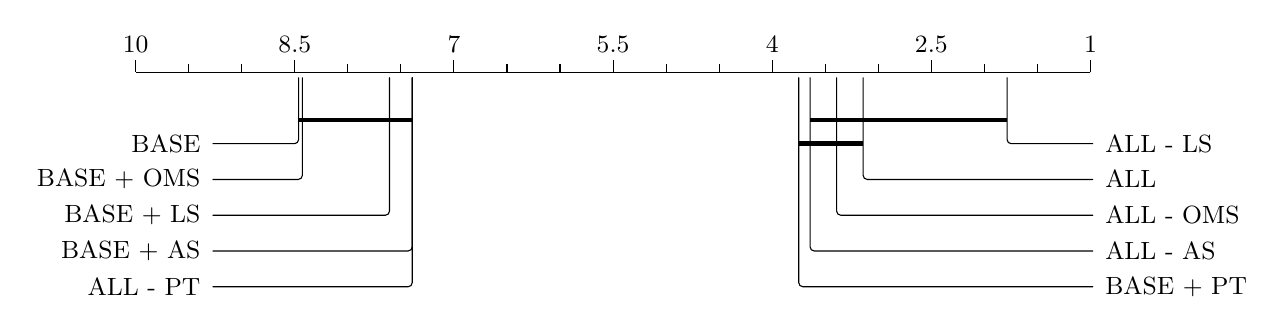
\begin{tikzpicture}[
  treatment line/.style={rounded corners=1.5pt, line cap=round, shorten >=1pt},
  treatment label/.style={font=\small},
  group line/.style={ultra thick},
]

\begin{axis}[
  clip={false},
  axis x line={center},
  axis y line={none},
  axis line style={-},
  xmin={1},
  ymax={0},
  scale only axis={true},
  width={\linewidth},
  ticklabel style={anchor=south, yshift=1.3*\pgfkeysvalueof{/pgfplots/major tick length}, font=\small},
  every tick/.style={draw=black},
  major tick style={yshift=.5*\pgfkeysvalueof{/pgfplots/major tick length}},
  minor tick style={yshift=.5*\pgfkeysvalueof{/pgfplots/minor tick length}},
  title style={yshift=\baselineskip},
  xmax={10},
  ymin={-6.5},
  height={7\baselineskip},
  xtick={1.0,2.5,4.0,5.5,7.0,8.5,10.0},
  minor x tick num={2},
  x dir={reverse},
]

\draw[treatment line] ([yshift=-2pt] axis cs:1.7857142857142858, 0) |- (axis cs:0.9523809523809524, -2.0)
  node[treatment label, anchor=west] {ALL - LS};
\draw[treatment line] ([yshift=-2pt] axis cs:3.142857142857143, 0) |- (axis cs:0.9523809523809524, -3.0)
  node[treatment label, anchor=west] {ALL};
\draw[treatment line] ([yshift=-2pt] axis cs:3.392857142857143, 0) |- (axis cs:0.9523809523809524, -4.0)
  node[treatment label, anchor=west] {ALL - OMS};
\draw[treatment line] ([yshift=-2pt] axis cs:3.642857142857143, 0) |- (axis cs:0.9523809523809524, -5.0)
  node[treatment label, anchor=west] {ALL - AS};
\draw[treatment line] ([yshift=-2pt] axis cs:3.75, 0) |- (axis cs:0.9523809523809524, -6.0)
  node[treatment label, anchor=west] {BASE + PT};
\draw[treatment line] ([yshift=-2pt] axis cs:7.392857142857143, 0) |- (axis cs:9.297619047619047, -6.0)
  node[treatment label, anchor=east] {ALL - PT};
\draw[treatment line] ([yshift=-2pt] axis cs:7.392857142857143, 0) |- (axis cs:9.297619047619047, -5.0)
  node[treatment label, anchor=east] {BASE + AS};
\draw[treatment line] ([yshift=-2pt] axis cs:7.607142857142857, 0) |- (axis cs:9.297619047619047, -4.0)
  node[treatment label, anchor=east] {BASE + LS};
\draw[treatment line] ([yshift=-2pt] axis cs:8.428571428571429, 0) |- (axis cs:9.297619047619047, -3.0)
  node[treatment label, anchor=east] {BASE + OMS};
\draw[treatment line] ([yshift=-2pt] axis cs:8.464285714285714, 0) |- (axis cs:9.297619047619047, -2.0)
  node[treatment label, anchor=east] {BASE};
\draw[group line] (axis cs:7.392857142857143, -1.3333333333333333) -- (axis cs:8.464285714285714, -1.3333333333333333);
\draw[group line] (axis cs:1.7857142857142858, -1.3333333333333333) -- (axis cs:3.642857142857143, -1.3333333333333333);
\draw[group line] (axis cs:3.142857142857143, -2.0) -- (axis cs:3.75, -2.0);

\end{axis}
\end{tikzpicture}